\chapter{Maximum Likelihood Estimator}
\label{ch:MLE}
\section{Overview}
The path of the Cosmic Microwave Background (CMB) photons gets bent due to the intervening galaxy cluster. 
Distortion in the background CMB is of the order of few arcminutes for a massive galaxy cluster.
On the galaxy cluster length scales (order of arcminutes) CMB can be approximated as a gradient due to diffusion damping \citep{silk96}. 
Gravitational lensing induces a dipole kind of structure on top of the gradient with hot and clod spots swapped. 
The strength of the gravitational lensing signal (lensing dipole) is directly proportional to the background gradient and the cluster mass. 
As polarisation signal is an order of magnitude smaller than temperature, lensing signal in polarisation is also an order of magnitude smaller than that of temperautre. 
Fig ~\ref{fig:lensing_signal} shows the lensing signal for a cluster of mass $5*10^{14}$ $M_{\odot}$ and at redshift of $z$ = 0.7.
On the left panels we have the background CMB gradient for the temperature and polarisation stokes Q and U parameters, on the middle panel we have the corresponding lensed maps; on the right panel we have the lensing dipole signatures.

Lensing remaps the unlensed CMB temperature and polarisation fields based on the gravitational deflection angle of the cluster. 
\begin{eqnarray}
T(\hat{n}) = \tilde{T}(\hat{n} + \alpha(\hat{n}))\\
Q(\hat{n}) = \tilde{Q}(\hat{n} + \alpha(\hat{n}))\\
U(\hat{n}) =  \tilde{U}(\hat{n} + \alpha(\hat{n}))
\end{eqnarray}
where T represents the temperature field, Q and U are the stokes polarisation parameters respectively. 
Tilde represents the unlensed fields, $\alpha(\hat{n})$ is the deflection angle vector due to the cluster lensing along the $\hat{n}$ direction. 
Deflection angle is related to gravitational potential as $\nabla \phi (\hat{n})$ and is directly proportional to the mass of the cluster.

In literature, there are several methods to extract lensing singal from CMB data. 
During my thesis, I mainly worked on two methods for extracting lensing signal from the observed CMB data: Maximum Likelihood Estimator (MLE) and Quadratic Estimator (QE). 
In this chapter, I will explain the MLE in detail. While we compare the results of MLE with QE, QE is explained in detail in next chapter.
\begin{figure}[t]
\begin{center}
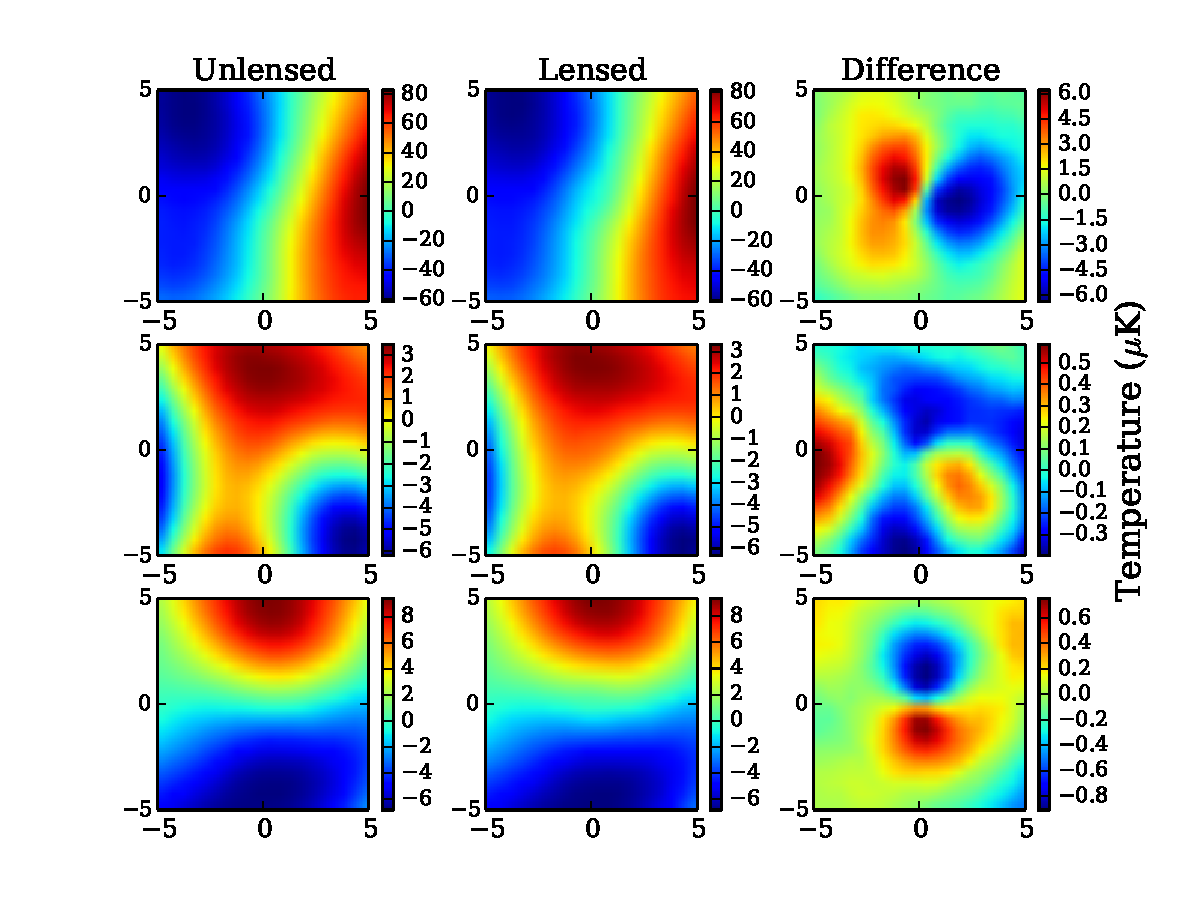
\includegraphics[width=\linewidth, keepaspectratio]{figs/lensing_signal.pdf}
 \caption{Lensing effect on CMB due to a galaxy cluster of mass $5\times 10^{14}$ \msolar.
  On the top panel we show the effect of cluster lensing on CMB temperature field.
  Bottom two panels are for the stokes Q and U parameters. 
 } 
\label{fig:lensing_signal}
\end{center}
\end{figure}

\section{Maximum Likelihood Estimator}
\label{sec_MLE}
Gravitational lensing by a galaxy cluster induces extra pixel-pixel correlations. 
MLE extracts the lensing signal by modeling these pixel-pixel correlations in the form of covariance matrix.


\subsection{Covariance matrix calculation}
Here, I explain the calculation of covariance matrix which will act as the model.
The distortion of CMB due to a galaxy cluster is of the order of arcminutes; much of the lensing is within 10\am from cluster center.
For covariance matrix calculation we take central \smallboxsize cutout.
We also checked that by increasing the boxsize to 14\am we gain an improvement in a SNR of less than 1\%, however, that the increases the computational complexities. 


 We calculate the covariance matrix by using a set of simulated skies. 
 To calculate the simulated lensed CMB sky, first we generate the large-scale structure lensed CMB power spectra ($C^{TT}_{l}, C^{TE}_{l}, C^{EE}_{l},$ and $C^{BB}_{l}$) form CAMB for the $planck$ 2015 cosmology \citep{planck15_13}.  
 We generate Gaussian random realisations with these power spectra on a 50\am X 50\am box. 
 Q and U maps are generated by using E and B maps as
 \begin{eqnarray}
Q = E + B\\
U = E + B
 \label{eq:coord_trans}
 \end{eqnarray}
 
 \pending{correct the equations}
 While we only use  \smallboxsize  for final calculations we simulate a bigger box (50\am) to take into account the large scale gradient.
 These Gaussian realizations are then lensed by an assumed galaxy cluster density profile (explained in next section). 
 
 With simulated lensed CMB maps in hand we calculate the covariance matrix as follows
 \begin{eqnarray}
\Sigma_{lens}(M,z) & = & \left<(\textrm{\textbf{G}} - \left<\textrm{\textbf{G}}\right>) (\textrm{\textbf{G}} - \left<\textrm{\textbf{G}}\right>)^{T}\right>\\
  =   \frac{1}{n-1}\sum\limits_{i = 0}^{n} (\textrm{\textbf{G}}_{i} - \left<\textrm{\textbf{G}}\right>) (\textrm{\textbf{G}}_{i} - \left<\textrm{\textbf{G}}\right>)^{T} %(\textrm{\textbf{G}}_{i} - \left<\textrm{\textbf{G}}\right\
%s>)^{T},
\label{eq_lensed_cmb_cov_mass_z}
\end{eqnarray}
 where vector $G_{i}$ is either the polarisation or temperature simulated data for $i^{th}$ sky realisation. 
 The number simulated skies depend on the number of degrees of freedom in the covariance matrix. 
 In our case, we concatenate Q and U maps for our polarisation estimator for which the covariance matrix is a 800 X 800 matrix. 
 Number of simulations scale as twice the number of elements in the covariance matrix; we found 1,30,000 simulations are sufficient for recovering cluster masses without any bias. 
  We then multiply Hartlap correction term $\frac{(n_{sims} -n_{d} -1)}{n_{sims}}$, where $n_{sims}$ is 1,30,000 and $n_{d}$ is the length of the vector 400(800) for T(QU), to remove any possible bias in $\Sigma^{-1}_{lens}$ due to the limited number of simulations. 
  
 We also use these simulated skies to quantify the effects of statistical and systematic uncertainties.
 There are several astrophysical sources which act as a systematic bias and foregrounds for the CMB-cluster lensing analysis. 
 In this work we consider clusters own SZ effects such as thermal Sunayev-Zel'dovich (tSZ) and kinematic Sunayev-Zel'dovich effects. 
 %tSZ is in explained in detail in the next chapter. 
 Along with these SZ effects we have also considered sources which are uncorrelated with cluster such as tSZ effect from other halos, dusty star forming galaxies (DSFGs), and radio galaxies.
 In appendix, we provide in more details about the addition of these foregrounds to simulated skies.
 
 In this chapter we have considered only simulated data to check the efficiency of MLE. 
 Unless otherwise mentioned all the clusters are simulated at a mass of $M_{200} = 2*10^{14}$\msolar \pending{footnote} and at redshift of 0.7.
 For covariance matrix calculation we simulate the skies at redshift of $0.7$ with mass resolution of $2*10^{12}$\msolar. 
 Note that such fine gridding might not be computationally feasible for data where the clusters span wide range of masses and redshifts.
 An optimal solution would be generate the covariance matrices on coarser grid of mass and redshift and then interpolating it on a finer grid.
 
 
 
  
   
  
  \subsection{Likelihood Estimation}
  With the covariance matrix in hand we calculate the likelihood given the data as follows 
  
  \begin{equation}
  -2lnL(d|\Sigma_{lens}) = ln |\Sigma_{lens}| + d^{T} \Sigma^{-1}_{lens} d
  \end{equation}
  where the data vector $d$ is the pixel values of the observed T or Q/U maps.
  The pixel values are defined as the variations from the mean CMB temperature (polarisation) and hence have zero mean.
  
  %Since the majority of the lensing singal is within few arcminutes from the cluster center, we carry out the lensing analysis within \smallboxsize of the cluster center to simplify and speed up the analysis. 
  %We also checked that by increasing the boxsize to 14\am we gain an improvement in a SNR of less than 1\%, however, that the increases the computational complexities. 
  As pointed out earlier, the lensing signal of a single galaxy cluster is much weaker to be detected. 
  We stack many clusters to increase SNR (signal to noise ratio) to a reasonable level
  \begin{equation}
  -2ln L(d| \Sigma_{lens})_{tot} = \Sigma^{n}_{i =0} w_{i} [ln |\Sigma_{lens}| + d^{T}_{i} \Sigma^{-1}_{lens}  d]
  \end{equation}
  where n is the total number of clusters in the sample, $w_{i}$ is the weight for the $i^{th}$ cluster which depends on the survey noise etc.. 
  In this chapter as we are using simulated clusters, we assign uniform weights to each cluster.  

  \subsection{Lensing convergence profile}
  In order to lens the simulated CMB sky we need to know the lensing deflection angle.
  Deflection angle depends on the lensing convergence profile as follows:
\begin{equation}
 \alpha = \nabla. k = -\nabla^{2} \phi
 \end{equation}
 where $\alpha$ is the deflection angle, $k$ is the lensing convergence profile, and $\phi$ is the lensing potential.
 For a symmetrical density profiles, the lensing convergence profile is equal to the ratio of surface mass density over the critical density of the Universe at the cluster redshift $k = \frac{\sigma(x)}{\sigma_{crit}}$.
 
The surface mass density or also know as the projected mass density of the halo is obtained by integrating the halo density profile along the line of sight. 
 \begin{equation}
 \sigma(x) = 2 \int^{\inf}_{0} \rho(r) ds
 \label{eq:surface_density}
 \end{equation}
 where r is the radial distance, x is the corresponding 2D planar distance and s is distance along the line of sight with s =0 being the plane of the cluster.
 The critical surface density of the Universe at cluster redshift is given by
 \begin{equation}
 \sigma_{crit} = \frac{c^{2}}{4\pi G} \frac{D_{cmb}}{D_{clus}D_{cmb,clus}}
 \end{equation}
 where $D_{cmb}$ is the comoving distance to the epoch of recombination (z= 1100), $D_{clus}$ is the comoving distance to the cluster (in our case comoving distance to the redshift), and $D_{cmb,clus}$ is the comoving distance between the CMB and the cluster.
 
 Unless otherwise mentioned, I define all the cluster quantities in the chapter with respect to $R_{200}$, which is defined as the radius within which the mean cluster density is 200 times the Universe critical density at cluster redshift $\rho^{z}_{crit}$. $M_{200}$ will be 
 \begin{equation}
 M_{200} = \int^{R_{200}}_{0}  4\pi x^{2} \rho(x) dx
 \end{equation}
 By definition $M_{200}$ is also given by
 \begin{equation}
 M_{200} = \frac{800\pi}{3} R^{3}_{200} \rho^{3}_{crit}
 \end{equation}
 
 The above mathematical equations hold for any spherically symmetric halo, now we move on to a specific case of Navarro Frenk White (NFW) halo density profile.
 In the NFW profile, the density of the dark matter halo as function radius is given by:
 \begin{equation}
 \rho(r)= \frac{\delta_{c}\rho^{z}_{crit}}{(\frac{r}{R_{s}})(1+\frac{r}{R_{s}})^{2}}
 \end{equation}
 where $\delta_{c}$ is the characteristic over-density, $R_{s}$ is the characteristic scale radius, and $c$ is the dimensionless concentration parameter.
 The dimensionless over-density is given by $\delta_{c} = \rho_{0}/\rho^{z}_{crit}$, where $\rho_{0}$ is the cluster central density and  $\rho^{z}_{crit}$  is the crititcal density of the universe at cluster redshift.
 Plugging the above equation in ~\ref{eq:surface_density}, we get the surface density for the NFW halo. 
 By slightly change the variables of integration as $s=\sqrt{r^{2} - x^{2}}$ and $ds = \frac{rdr}{\sqrt{r^{2} - x^{2}}}$ we obtain:
 \begin{equation}
 \Sigma(x) = 2\delta_{c} \rho^{z}_{crit} R^{3}_{s} \int^{\inf}_{x} \frac{1}{r(R_{s} + r)^{2}} \frac{rdr}{\sqrt{r^{2} - x^{2}}}
 \label{eq:sr_den}
 \end{equation}
 The scale radius is related to the concentration parameter as follows:
 \begin{equation}
 c = \frac{R_{200}}{R_{s}}
 \end{equation}
 In this chapter we have set $c = 3.0$ following \cite{bhattacharya13}.
 The ~\ref{eq:sr_den} can be solved analytically and the explicit closed-form expression for the NFW case has been given by \cite{bartelmann96}.
 Unless otherwise mentioned we consider the galaxy clusters to follow NFW profile, however,  the mathematical framework described above can be applied any halo density profile. 
 
 
 \section{Results}

 In this section first we validate our pipeline using simulations, we report the expected mass uncertainties for the polarisation and temperature MLE. 
 Then we compare the performance of MLE and QE for ideal simulations by only vary the experimental noise levels and not including any galactic or extra galactic foregrounds. 
 Later, we compare the performance of the estimators in the presence of foregrounds. 
 In this chapter all the results are for a set of 100,000 simulated clusters (expected number of clusters for CMB-S4) each at a mass of $2\times10^{14} M_{\odot}$ and at redshift of 0.7.
 To obtain the lensing significance, we calculate the ratio of combined likelihood at zero mass to that of maximum likelihood:
 \begin{equation}
 \lambda = \frac{L (M_{200} =0)}{max(L(M_{200}))}
 \end{equation} 
 According the Wilk's theorem, in many cluster limit $\lambda $ follows chi-square statistic with one degree of freedom ($M_{200}$ in our case).
 The detection significance reported in this chapter is equal to $-2 ln (\chi)$
 Similarly, we obtain the errors on mass estimate by calculating masses at which $-2lnL(M_{est}) + 2 ln L (M_{200})$ is equal to 1, where $M_{est}$ is the best fit mass.
 
 
 \subsection{Ideal simulations}
 There are two main purposes for our ideal simulations. 
 Firstly, ideal simulations serve as benchmark to estimate the effect of different systematic and statistical sources of uncertainties on our lensing analysis. 
 In addition to that, it provides equivalent conditions to allow for a fair comparison between MLE and QE.
 To validate the pipeline we simulated 100,000 galaxy clusters each at a mass of $2*10^{14} M{\odot}$ and at redshift of $z = 0.7$; later we added white noise realisation at 1\ukam.
 In the top panel of Fig 1, the black solid line represents the combined likelihood for temperature MLE estimator, solid orange curve is that for the polarisation QU estimator and the dashed orange curve is for EB estimator. 
 We calculated the detection significance as mentioned above, lensing signal detected at 400$\sigma$ and 110$\sigma$ for temperature and polarisation MLE respectively. 
 Null test results are shown in bottom panel of Fig. 1, for which we turned of lensing in our pipeline.
 As expected for all the three MLE estimators (T, QU, and EB) the likelihoods peak at zero mass.
 
 \begin{figure}[t]
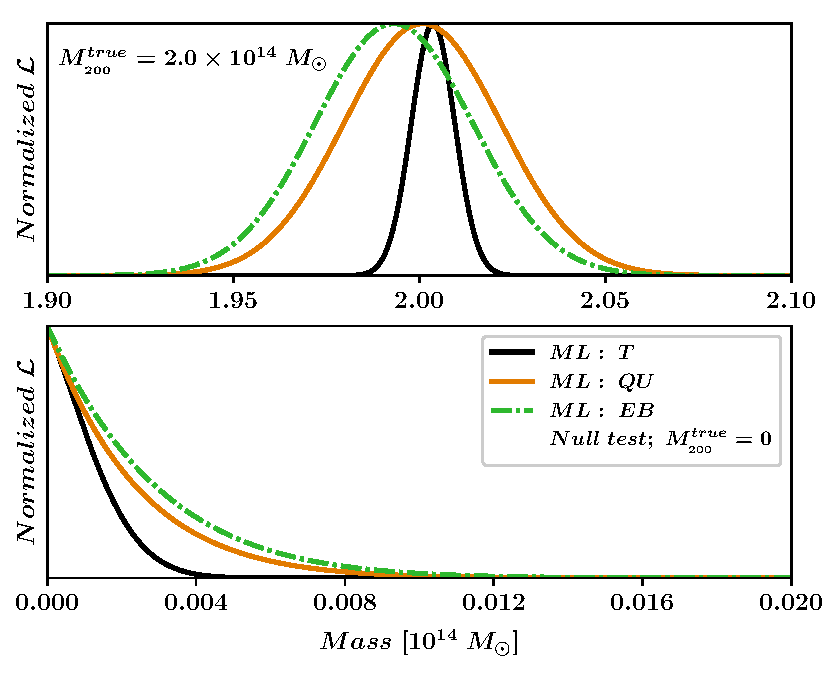
\includegraphics[width=\linewidth, keepaspectratio]{figs/fig0-eps-converted-to.pdf}
 \caption{In the top panel we show the combined likelihood of 100,000 clusters each at redshift of 0.7 and at mass of $2\times 10^{14} M_{\odot}$ for temperature and polarisation MLE estimators. The difference between QU and EB estimator isn't statistically significant. In the bottom panel we show the results of null test and as expected the likelihood peaks at zero for all three estimators}
 \end{figure}
 
 In the left panel of figure 2., we compare the performances of all three MLE estimators and the temperature QE estimator as function of experimental noise levels. 
 %Note that, no galactic or extra galactic foregrounds are added. 
 %All the fractional mass uncertainties are stated for 100,000 clusters each at a mass of $2\times 10^{14} M_{\odot}$ and at a redshift of 0.7.
 It is evident from the figure that in the absence of foregrounds, temperature outperforms polarisation above noise-level of 0.075 \ukam.
 So even for future CMB-S4 experiment temperature has to be the primary channel from pure SNR perspective.
 Only below noise-level of  0.075 \ukam, polarisation starts competing with temperature.
 As pointed out earlier, the lensing signal is directly proportional to the background CMB gradient, gradient in polarisation is 10$\times$ smaller than that of temperature as shown in ~\ref{fig:lensing_signal}. However, below noise-level of 0.075\ukam the CMB temperature background gradient acts as a source of noise. 
 
 Orange squares and green circles represent MLEs using polarisation QU maps and EB maps respectively. 
 As expected, there is no significant differences between their performance from a theoretical standpoint. 
 The apparent difference at higher experimental noise levels is not statistically significant.
 However, using QU maps simplifies the analysis as these modes are directly measured by the experiment and doesn't involve co-ordinate transformation ~\ref{eq:coord_trans}. In this chapter, I have considered only $QU_{MLE}$ polarisation estimator.
 
  
 Lastly, we compare the performance of temperature MLE (solid black triangles) and QE (orange solid squares). 
 QE is a first order approximation of MLE.
 %While both temperature MLE and QE perform equally well at higher noise levels, MLE has clear advantage over QE at low noise levels.
 At higher noise levels (low SNRs) the effect of higher order terms is negligible, hence no difference between the performance of MLE and QE estimators.
 However, at low noise levels (high SNRs) MLE outperforms QE. 
  Though not show here, there is no difference between polarisation MLE and QE for the range of the experimental noise we have considered.
  This is not surprising as polarisation lensing SNR is low for the considered noise levels.
 
 The effect of higher order terms can be recovered using an iterative version of QE as shown in \cite{Yoo and Zaldarriaga}.
 We find that MLEs performance is improves by a factor of 2 at noise level of 0.1\ukam  for our fiducial sample of 100,000 clusters each at  $M_{200} = 2 \times 10^{14}$ \msolar and redshift of 0.7. 
  
Both MLE and QE estimators share a common difficulty in regards with the assume cluster density profile.
This dependence shows up in different places in each estimators.
 \begin{itemize}
 \item In MLE as explained in ~\ref{sec_MLE} we fit the lensed CMB templates to the observed data. The lensed CMB templates are obtained by assuming a cluster density profile. 
 \item QE works by the exploiting the correlation between the background CMB gradient and lensing dipole to obtain lensing convergence profile. 
 We fit models to these lensing convergence profile to extract the mass of the cluster.
 
 \end{itemize}
There is no reason not take advantage of the improved performance of MLE over QE at low experimental noise levels. 
 \begin{figure}[t]
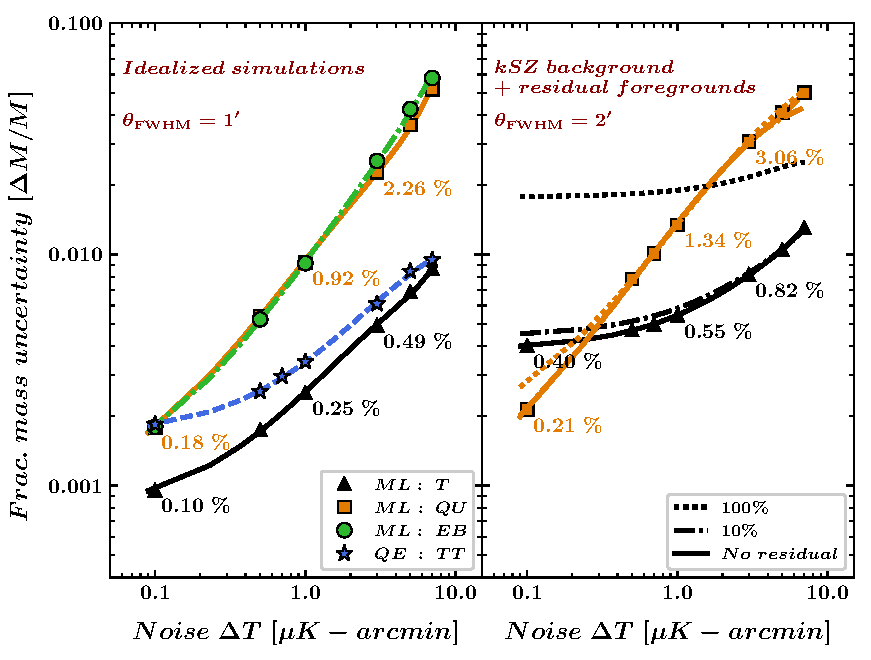
\includegraphics[]{figs/fig1-eps-converted-to.pdf}
 \caption{In the left we show the performance of different estimators for idealised simulations as function of experimental noise levels. We consider the effects of various foregrounds on the estimators in the right panel. All the curves are for a set of 100,000 clusters each at mass of $2\times 10^{14} M_{\odot}$ and at redshift of 0.7.}
 \end{figure}
   
   \subsection{Effects of extragalactic foregrounds on lensing analysis}
   In this section, we look into the effects of extragalactic foregrounds on lensing analysis. While galactic foreground also affect the lensing analysis, however, by using a combination of frequencies we can suppress galactic foregrounds. The bias due to some of the foregrounds such as cluster's own SZ effect etc., are reported in the next section. Here we are only concerned about the additional noise due to extra galactic foregrounds. The level of foregrounds is much higher in the temperature than in the polarisation channel, hence the effect of foregrounds is higher in temperature estimator than polarisation. We consider the impact of tSZ, kSZ, radio galaxies and dusty galaxies on the 150GHz channel.
   
   The impact of foregrounds on the performance of lensing estimators as function of experimental noise level is shown in fig. 2. 
   As expected foreground negligibly effects the polarisation channel (orange squares).
   For the temperature estimator the extragalactic foregrounds set an effective noise level of 5\ukam if not cleaned, this results in plateauing of 1.8\% in mass uncertainty (black dotted line). 
   Without any foreground cleaning polarisation QU estimator outperforms the temperature channel at 1.5 \ukam.
 However, we can exploit the frequency dependence of various extragalactic foregrounds to reduce the effect of foregrounds.
 While combining multiple frequency channels we assume that the beam size is 1\am  irrespective of the frequency to simplify the analysis. 
Using different spectral dependence of background CMB and tSZ we can completely eliminate the tSZ power.
 However, kSZ has the same spectral dependence as that of the CMB and hence cannot be eleminated. 
 The black solid triangles repersent the performance of temperature estimator 100\% kSZ and no tSZ, radio or dusty galaxies.
 The dashed solid line corresponds to 10 \% of radio and dusty galaxy power, 100\% of kSZ power and no tSZ power. 
 With 90\% cleaning of foreground, temperature estimator becomes the main channel for estimating lensing signal even for the proposed CMB-S4.
  There is only a fractional improvement in the performance above 90\% of cleaning. 
  It is important to note here that foreground cleaning enlarges the beam which is not taken into account here, which will degrade the mass uncertainties even further.
  
  To summarize, the extragalactic foreground almost have no effect on the performance of polarisation estimators. 
  On the other hand, temperature estimators will have effective noise floor of 5\ukam if foregrounds aren't taken into account. 
  As we will see in next in addition to increasing final mass uncertainties, some of these foregrounds will also acts sources of systematic bias.
  
  \section{Systematic bias checks}
  From figure 1, it is evident that we will achieve less than 1\% mass uncertainty for a CMB-S4 kind of experiment. 
  However, we need to account for all the systematic biases to claim our sub-percent mass measurements.
    In this section, we quantify various sources of systematics that could bias our final results.
    We examine the following sources:
    \begin{itemize}
    \item error in cluster center
    \item differences due to the cluster density profile
    \item other halos along the line of sight
    \item error in redshift
    \item cluster's tSZ effect
    \item cluster's kSZ effect
    \item dusty galaxies
    \end{itemize}
    The last three sources negligibly affect the polarisation estimators as they are only partially polarised. 
    Note that all these sources may effect polarisation and temperature estimators to different extents due to differences in the mode weighing between estimators.
     
 The baseline simulations for bias calculations include 1 \am Gaussian beam, experimental noise level of 1\ukam (which corresponds to a noise level of $\sqrt{2}$\ukam in polarisation) and no foreground unless otherwise stated.
  The amount of bias depends on experimental beam size, noise-level, and foregrounds as they define the weighing of different angular scales of MLE. 
  However, this section will roughly quantify the magnitude of bias and give a direction to pursue future work in CMB-cluster lensing to reduce the systematic uncertainties. 
   We report the systematic bias for a sample of 1,000,000 clusters each at a mass of $2 \times 10^{14}$ \msolar and each at a redshift of 0.7 (expect for redshift uncertainty case). The bias is calculated as follows:
   \begin{equation}
   b = \frac{M_{bias}}{M_{true}} - 1.
   \end{equation}
   where $M_{bias}$ is the final recovered mass when the source of bias of bias is included in the lensing analysis and $M_{true}$ is the input mass. 
   Error in the bias is obtained by calculating the scatter in 100 subsamples.
   
   We report the magnitude of bias for all the sources considered in table 1. 
 Other than errors in redshift, all other sources of bias should be considered carefully to achieve sub-percent uncertainty as claimed for CMB-S4 experiment. 
 Here we have not considered surveys specific systematics such as false detections, selection function, and projection effects or some form of bias in weighing the clusters.
 
 \subsection{Halos along the line of sight}
 In reality the final estimated mass also depends on other halos present along the line of sight and on the correlated halos. 
 If the effect due to these halos aren't taken into account then the final results will be biased high. 
 This is particularly a major concern for low mass haloes as they won't be detected by the survey/
 To quantify the effect of this bias we look into Flender et al simulation. 
 It is an N body cosmological simulation with 17 million objects; for cluster we random select a halo within a mass range of  $M_{200} \in$ [1.8, 2.2] $10^{14}$\msolar and redshift range of [0.6,0.8].
We simulate the CMB maps as explained earlier, however, instead of lensing the CMB with just the cluster convergence profile we lens it the all the convergence profiles which are within the 50\am of the cluster center. 
Analysis proceeds normally after this - these lensed CMB maps are convolved by Gaussian beam after which specified white experimental noise is added. 
As expected both polarisation and temperature estimators are biased high : 2.5 $\pm$ 0.3\% for temperature MLE and 6.3 $\pm$ 1.1\% for polarisation QU estimator.
We can reduce the bias by taking two halo term into account, however, that will include more nuisance parameters increasing the statistical uncertainty of the final results. 
Galaxy clusters are not isolated objects, they are generally found in large scale filaments. 
Also, clusters with ellipticity along the line of sight have higher tSZ increasing the probability of their detection. 
They are also likely to be found in filaments, resulting a high bias; however, the scope of finding the bias due to the large filaments is outside the scope this thesis. 
Its worth noting that in order to fully realise the potential of CMB-S4 in obtaining sub-percent mass uncertainties we need to work on systematics.
Accurate and reliable simulations of structure formation on large volumes is needed in order to handle this source of systematic error at the sub-percent level.

\subsection{Cluster mass profiles}
As mentioned earlier both QE and MLE assume a density profile, however, this may not be the true cluster profile. 
Any difference between the assumed mass profile and true cluster profile will bias the final results.
In all the above results we assumed clusters to follow NFW profile. 
However, studies have shown that for massive clusters the density profile deviates significantly from NFW at radius r $\ge$ 0.5 $R_{200}$. 
It is unknown whether these deviations will be larger or smaller for lower mass clusters.
In addition to this, a recent study has shown that for analysis involving stacked halos Einasto profile provides a better estimate.
Here we consider three density profiles in order to estimate the bias.
\begin{itemize}
\item A modified version of the NFW profile which drops off more rapidly with radius
\begin{eqnarray}
\kappa_{\rm NFW}^{mod}(x) =
\begin{cases}
    \kappa_{\rm NFW} &; x \le 0.75\theta_{_{200}}\\
    \kappa_{\rm NFW} \times m(i,j)&; 0.75\theta_{_{200}} < x \le 1.5\theta_{_{200}}\\
    0 &; otherwise
\label{eq_kappa_mod}
\end{cases}
\end{eqnarray}
where $m(i,j)$ is a Hanning 2D apodization kernel.
We create the 2D apodization kernel as $m(i,j) = m(i) \times m(j)$ with $m(i) = \frac{1}{2} \left[ 1 - cos\left(\frac{2\pi  (i-n/2) }{n} \right)\right]$, where i and j are pixel indices in the $n \times n$ map.
\item A change to the cuspiness of cluster core in the NFW profile, following \citet{king2001} 
\begin{eqnarray}
\kappa_{\rm NFW}^{sub}(x)  & =  &
\begin{cases}
    \kappa_{\rm NFW}\ + \sum\limits_{i=1}^{3} \kappa_{sub}^{i}&; x \le 1'\\
    \kappa_{\rm NFW} &; otherwise;
\label{eq_kappa_sub}
\end{cases}
\end{eqnarray}
\item The Einasto profile \citep{einasto1989}
\begin{eqnarray}
\rho(r)_{_{Ein}} & = &  \rho_{_{0}}\ exp\left( - \frac{2}{\alpha} \left[\left(\frac{r}{R_s} \right)^{\alpha} - 1\right]\right)
\label{eq_einasto_density}
\end{eqnarray}
with the shape parameter $\alpha = 0.18$ \citep{ludlow2013}. The convergence profile for this profile is obtained by inserting this into int\
o Eq.(\ref{eq_surface_denisty_los_integral}).
\end{itemize}
 
 In each of the three cases we lens CMB by the assumed cluster profile, however, we use NFW profile to calculate our model.
 Assuming wrong cluster profile will bias the results from -2.5\% to 3.8\% as shown in Table 1. 
 A similar study was done in optical weak-lensing analysis where they used NFW profile in the model and Einasto profile in the simulated data; they found a bias of -2 to 7 \% depending on the cluster mass. This level of bias is larger than the statistical mass uncertainties expected for the CMB-S4 experiment, and a significant challenge for upcoming experiments.
More work will be required to accurately measure the cluster mass profiles as a function of radius if we are to achieve the full potential of galaxy cluster cosmology. 

\subsection{Cluster miscentering}

Any difference between the true cluster center and the model will result in a bias.
 Misestimation of the cluster center even by a small amount results in underestimation of cluster mass as we loose some of the lensing signal.
To quantify the effect of miscentering, we draw an offset between from normal distribution N(0, $\sigma^{2}$) and lens the CMB with offseted clusters to obtain simulated data, however, model doesn't take the offset into account.
Fig 24 shows the bias in the final results as a function of offset for both temperature (orange squares) and polaristion estimators (black triangles).
As expected the bias increases with rms of the offset, the positive bias at very low offsets is not statistically significant.
Temperature estimator draws more information from smaller angular scales than the polarisation estimator, hence the bias in temperature estimator is more compared to the polarisation. Note that the here we haven't considered foregrounds, considering foreground would decrease the weightage of smaller angular scales. For survey with higher experimental noise, larger beams and foregrounds the bias will decrease.

 
The typical offset between the SZ-centroid and the X-ray or brightest central galaxy (BCG) is of the order of 0.5 \am.
From the figure, for 0.5 \am offset the mass is underestimated by 7.5 $\pm$ 0.3 \% for temperature estimator and 1.5 $\pm$ 1.3 \% for polarisation estimator. 
For a given constraint on the offset, a correction could be easily applied to eliminate the bias, however, that will result in a slight decrease of SNR.
Without considering the effect of foregrounds, we need to know the offset by 2\% (8\%) in order to achieve sub-uncertainty for future CMB-S4 survey.
However, adding foregrounds will reduce the weight of the information from smaller angular scales and lessen the requirement of how well the positional uncertainty must be known.
\begin{figure}[t]
\centering
%\hspace{-2mm}                                                                                                                               
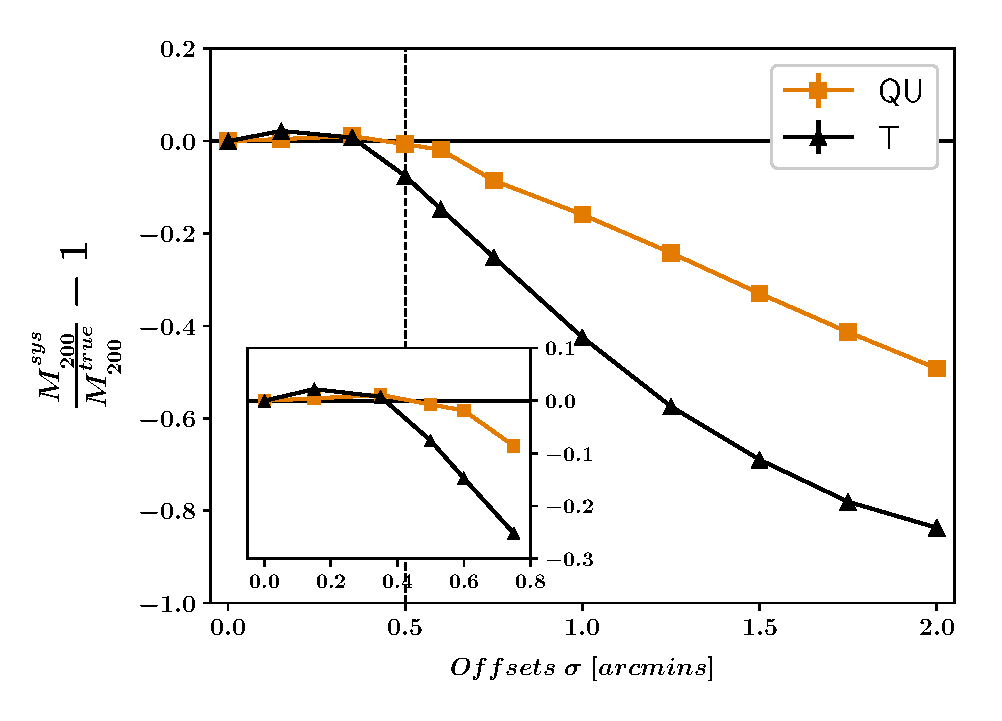
\includegraphics[width=0.85\textwidth, height=0.65\textwidth,clip=]{figs/fig2_v2.eps}
\caption{The low mass bias due to the positional offsets between SZ determined centroid and the true cluster center  for the $T_{\rm ML}$ (b\
lack triangles) and $QU_{\rm ML}$ (orange squares) estimators. The typical positional offset of $0.5'$ \citep{song2012} is marked with the v\
ertical dashed line. The error bars are derived using estimates gathered by repeating the test 100 times.}
\label{fig_sys_bias_cluster_offsets}
\vspace*{2mm}
\end{figure}


 \subsection{Redshift Bias}
CMB-cluster lensing can be used to calibrate the mass scaling relations of SZ surveys (SPT-3G, AdVACT, Simons Observatory etc.,), optical surveys (LSST, DES etc.,), and X-ray surveys (eRosita etc.,). These surveys are expected to return tens to hundreds of thousands of clusters, however, obtaining spectroscopic redshift for each cluster is not feasible.  
On the other hand, we can have red squence redshifts up to an higher redshift threshold and a redshift lower limit for clusters at even higher redshifts. 
The current state of the art for red sequence redshifts can be seen in the  DES \texttt{redMaPPer} catalog, where the \emph{photo-z} errors are $\sigma_{z} = 0.01 (1+z)$ for $z \le 0.7$ and $\sigma_{z} = 0.02 (1+z)$ for $z \sim 0.9$ \citep{rykoff2016}. The mass bias is estimated by considering a redshift scatter for individual clusters. We conservatively take the redshift errors to be
\begin{equation}\nonumber
\sigma_z = \left\{
\begin{array}{l}
    0.02 (1+z);  ~~z < 1 \\
    0.06 (1+z);  ~~z > 1
  \end{array}\right.
\end{equation}

We create mock lensed CMB maps using the true redshifts $z\in[0.5, 1, 1.5, 2]$ for the cluster. However, the `measured' redshift, $z + \sigma_{z}$, for each cluster is used to construct the pixel-pixel covariance matrix. The masses are then fit using this incorrect covariance mat\
rix, and the fractional bias determined.                                                                        
The case that should have the largest bias, $z=2$, is listed in Table~\ref{tab_sys_bias}. We do not detect a mass bias at any redshift. 
 
\subsection{kinematic SZ signal}
CMB photons get doppler shifted due to the relative motion of the galaxy cluster with respect to the CMB rest frame, this is know as kinematic Sunyaev - Zel'dovich effect (kSZ).
While kSZ is an order magnitude smaller than tSZ, unlike tSZ effect, kSZ effect has the same spectral dependence as that of CMB. 
We cannot combine multiple frequency channels to eliminate kSZ effect. 
Instead we can use polarisation estimator as, it is only partially polarised.

To quantify the kSZ bias, we consider the publicly available kSZ maps and halo catalog from Flender et al simulations.
These are full sky simulations in healpix pixelisation scheme with nside of 8192 correpsponding to 0.42 arcminute resolution.
Within a mass range of $M_{200} \in [1.8 \times 10^{14},2.2 \times 10^{14}]$ $M_{\odot}$ and redshift $\in$ [0.6,0.8] the catalog has 20,000 halos. 
For each cluster in the simulated data we randomly pick 50\am $\times$ 50\am cutout centered around the halo, smooth it with experimental Gaussian beam of FWHM = 1\am and add it to the lensed cluster cutout. 
Final results are significantly biased if the the kSZ effect is not taken into account while modeling the pixel-pixel covariance matrix: we obtain a low bias of 41\%.
We get similar large bias levels when we used an analytic modelling for the cluster kSZ signal instead of extracting them from N-body simulations. Modelling the optical depth of the clusters using the Battaglia \cite{nickb2016} profile and drawing the cluster velocities from a normal distribution $N(0, \sigma^{2})$ with scatter $\sigma = 350\ km/s$, we obtained a 32\% bias in the recovered lensing mass.
  
 If we take effect of kSZ while modeling the pixel-pixel covariance matrix then as expected we eliminate the bias. 
 However, we don't exactly know the kSZ effect of a single cluster. According to current estimates the uncertainty in kSZ prediction is 20\% for a single galaxy cluster. 
 The reason for the uncertainty is the complex cluster baryonic physics which is not very well understood. 
 To determine the bias that would result due to the uncertainty in kSZ effect, we included 20\% uncertainty in the modeling the pixel-pixel covariance matrix. 
 This results in a low bias of 7.5 $\pm $ 0.4 \%, bias can either be low or high depending on underestimation or overestimation of kSZ.
 Interpolating linearly between the kSZ uncertainty and the bias, we find that 2-3\% uncertainty in kSZ would lead to sub-percent bias. 
 Given the current uncertainties in kSZ estimation, it acts as a serious obstacle in using CMB-cluster lensing for future CMB surveys. 
 
 \subsection{Thermal Sunayev-Zel'dovich effect}
 
Here we give a brief review of Thermal Sunayev-Zel'dovich (tSZ) effect and is explained in detail in the next chapter.
CMB photons while passing through galaxy cluster are inverse compton scattered of high energetic electrons present in cluster's hot intra cluster medium.
This results in excess of photons at higher frequency and deficit of photons at lower frequency, this is known as tSZ effect.
tSZ effect is an order of magnitude greater than lensing signal and will induce significant statistical and systematic uncertainties if not taken into account.
In the next two chapters we discuss in detail the methods through which we eliminate the tSZ bias in QE estimator.
Here, we quantify the tSZ bias in the MLE and discuss the methods that can be used to reduce the bias.
We consider two different approaches:
\begin{itemize}
\item use frequency channels to eliminate the tSZ
\item model the tSZ effect in the pixel-pixel covariance matrix
\end{itemize}
In an ideal world both of these approaches should completely eliminate the bias, however, due imperfect knowledge in the instrument calibration or the model will result in a bias. 
To evaluate the performance of each approach,  we use Compton $y$ maps produced on a $5^{\circ} \times 5^{\circ}$ box at resolution $2.'5$ from the smoothed-particle hydrodynamics (SPH) simulations of  \citet{mccarthy2013}.
Neglecting relativistic corrections, we convert the Compton $y$ maps into tSZ maps by
\begin{eqnarray}
\Delta T = y T_{\rm CMB} \left[x \left(\frac{e^{x/2} + e^{-x/2}}{e^{x/2} - e^{-x/2}}  \right)\right]
\end{eqnarray} where $x = \frac{h\nu}{k_{\rm B}T_{\rm CMB}}$, $\nu$ is the frequency in GHz, $T_{\rm CMB} = 2.73\ K$, $k$ is the Boltzmann constant, and $h$ is the Planck constant.

\subsection{tSZ frequency cleaning}
 Using the spectral dependence of tSZ we can eliminate it by using CMB maps observed at different frequency channels.
 In this chapter we assume the CMB is observed at 90 GHz and 150 GHz channels with Gaussian beam of FWHM 1.7\am and 1\am respectively.
 The tSZ amplitude at 90 GHz is 1.67 times that of 150 GHz.
 tSZ free map is obtained as follows:
 \begin{equation}
\widetilde{T}(\hat{\textbf{n}})  =  \frac{1.67\widetilde{T}_{{150}}(\hat{\textbf{n}}) - T_{{90}}(\hat{\textbf{n}})}{f-1}
\end{equation}
where
\begin{equation}
\widetilde{T}_{{150}}(\hat{\textbf{n}})  =  T(\hat{\textbf{n}})_{{150}} \ast \frac{B_{{90}}(\hat{\textbf{n}})}{B_{{150}}(\hat{\textbf{n}})},
\label{eq_smooth}
\end{equation}
 f is 1.67. It is important to note that 150 GHz has to smoothed with 90 GHz beam using \ref{eq_smooth} before subtracting out tSZ.
  For the analysis we have also assumed that the experimental noise level in both 90 and 150 GHz channels to be 1 \ukam. 
  Under these assumptions using tSZ free map will eliminate the bias (b = 0.0 $\pm$ 0.7), however, it will degrade the final SNR by a factor of three.
  In practice, it is unlikely to obtain a precise value of factor 'f' due the uncertainties in frequency band widths or errors in relative calibration of frequency bands.
  To evaluate the bias in the final results due to the uncertainties in the factor `f', we use simulations. 
  We assume an uncertainty of 1\% in f, which is overly conservative for future CMB surveys but comparable to that of current surveys.
 An error in f will result in leakage of tSZ in the final tSZ free maps and will bias the results.
 For 1\% uncertainty in `f' we find the final results to be biased low by -6.3 $\pm$ 0.7 percent. 
 The bias can shift depending on whether the SZ leakage is over estimated or under estimated.
  
tSZ has no power at 217 GHz and one might consider of using 217 GHz frequency channel instead of creating tSZ free maps. 
However, the power dusty galaxies are increase significantly with frequency.
So, the foreground power in 217 GHz channel is much more than 90 or 150 GHz channels. 
In addition to that, we should also take into account the contamination due to the correlation between the tSZ and cosmic infrared background due to these dusty galaxies.
 Current estimates find the correlation co-efficient to be $0.113^{+0.057}_{-0.054}$; estimating the tSZ-CIB signal at 220 GHz would yeild a signal nearly three quarters of the tSZ signal at 150 GHz. 
 In order to use 217 GHz channel, more work needs to be done in constraining the tSZ-CIB correlation.
 
 \subsection{tSZ fitting}
 Instead of removing the tSZ signal, one can include it in the pixel-pixel covariance matrix.
Following \S\ref{sec_kSZ_bias}, we calculate the expected tSZ contribution using SPH simulations from \citet{mccarthy2013}.
As would be expected, the bias is consistent with zero for perfect knowledge of the tSZ signal (b = $1.0 \pm 0.6\%$).
However, this bias increases quickly if the tSZ contribution is mis-estimated.
Analogously to the tSZ cleaning case, we would expect percent-level errors to lead to significant (order 6\%) biases.
Given that the current uncertainties in modeling the tSZ signal from galaxy clusters are more than an order of magnitude larger, it will be extremely challenging to achieve the sub-percent precision necessary to make this approach viable.
Another way is to tSZ model out of the 150 GHz channel.
 While this method doesn't degrade the SNR unlike the frequency cleaning, however, imperfect knowledge in theoretical modelling will result in a bias.
 
 
 \subsection{Dusty galaxies in the cluster and other foregrounds}
\label{sec_DG_sys_bias}


Galaxy clusters are known to host overdensities of dusty galaxies, with several papers measuring the resulting tSZ-CIB correlation \citep{actdunkley2013, george2015, PLANCKTSZCIB2016}.
We describe our modeling of these DG overdensities\footnote{For implementation reasons, in this section, we include all foregrounds mentioned in the Appendix \ref{sec_appendix}, even ones that are not cor\
related with the cluster itself, such as radio galaxies.} in the Appendix \ref{sec_appendix_extragal}.
If ignored, the tSZ-CIB correlation may substantially bias the recovered masses from temperature estimators, especially at higher frequencies.
The emission from dusty galaxies rises sharply with frequency, by an order of magnitude in $\mu K^2_{\rm CMB}$ from 90 to 150\,GHz and again from 150 to 220\,GHz.
Polarization estimators (at least at 150\,GHz and lower frequencies) are essentially unaffected due to the lower polarization fraction  of dusty galaxies (expected to be less than 4\% \citep{seiffert2007,sptpol_delensing_2017}).
The tSZ-CIB correlated power could be handled analogously to either the tSZ fitting or cleaning approaches in \S\ref{subsec:tszbias}.
However, a multi-frequency cleaning scheme will be less effective than for the tSZ effect since the spectral dependence of thermal dust emission varies between individual galaxies.
Here we look only at bias for the fitting approach where the extra pixel-pixel covariance due to the clustered dusty galaxies is folded into the likelihood.
The recovered mass is somewhat low: $b=4.5 \pm 1.7\%$.
The existence of a bias (higher than $2\sigma$) is slightly surprising since one would expect zero bias in the perfect information limit, and the significance is low enough that it may be a statistical fluke.
The dramatic increase in the uncertainty -- from 0.25\% to 1.7\% -- reflects the plateauing of the dotted line in right panel of Fig.~\ref{fig_delM_M_1000_clusters_T_QU_EB_ideal_FG}.
Unsubtracted foreground power effectively sets a lower bound on the instrumental noise.

\section{A look into the future}
\label{sec_forecast}

\begin{figure}
\centering
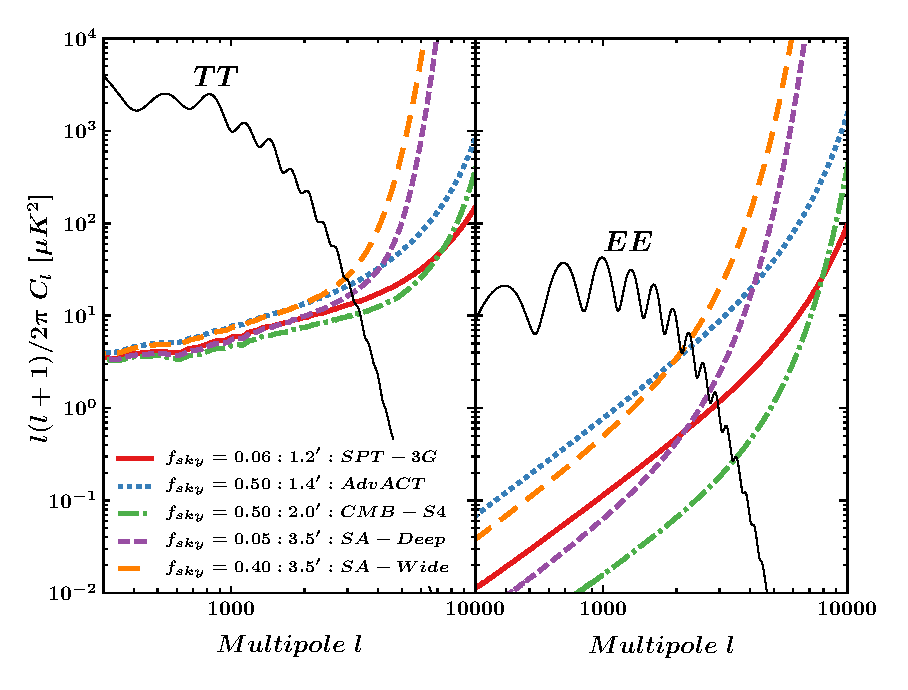
\includegraphics[width=1.\textwidth, height=0.68\textwidth,clip=]{figs/fig3.eps}
\caption{The expected residual foreground and noise power spectrum for the future CMB experiments.
The 90, 150, and 220 GHz channels have been combined using a constrained ILC technique to remove the tSZ effect while minimizing other extragalactic foregrounds and instrumental power.
The left and the right panels correspond to temperature and polarization respectively.
The plateauing of the residual temperature spectrum reflects the limited foreground removal possible with three frequency channels.
Specifications about each experiment are listed in Table \ref{tab_forecast_future_CMBexp}.}
\label{fig_ILC_res}
\end{figure}

In this final section we forecast the cluster mass uncertainties from CMB-cluster lensing for the AdvACT, Simons Array, and SPT-3G experiments, which we will collectively refer to as the Stage III experiments, \
and also for the proposed CMB-S4 experiment.
In addition to presenting the mass uncertainties for fiducial versions of these experiments, we examine how the mass uncertainty would change as a function of the beam size and map noise levels.
This information can be used to evaluate design tradeoffs while planning the CMB-S4 experiment.

\subsection{Expected lensing mass uncertainties for future CMB experiments}
\label{subsec:cmbs3s4}

We expect the next generation of CMB experiments, which will have substantially more detectors and a concomitant reduction in map noise levels, to dramatically improve the cluster mass calibration possible from\
 CMB-cluster lensing.
The experimental configuration of all the experiments considered is given in Table \ref{tab_forecast_future_CMBexp}.
Three options for telescope size (and therefore beam sizes) are listed for the proposed CMB-S4 experiment.
While current results have mass uncertainties of order $\ge 20$\% \citep{baxter2015,act_cmass2015,planckXXIV2015}, we expect Stage III experiments to reach 3\% and CMB-S4 to approach 1\%.

There are two reasons for the improvements.
First, with more detectors comes lower map noise levels (and larger survey areas).
The deepest current experiments reach approximately $5\,\mu$K-arcmin in temperature; the Stage III surveys  (AdvACT \citep{advact_2016};  Simons Array \citep{PB2_2016}, and SPT-3G \citep{benson2015_3g}) forecas\
t a few $\mu$K-arcmin; and projections for CMB-S4 are $\sim$\,1\,$\mu$K-arcmin.
Lower noise improves the lensing significance on any individual galaxy cluster.
Second, lower noise levels and larger survey areas translate into substantially more galaxy clusters.
Current ground-based SZ cluster catalogs have fewer than 1000 clusters \citep{ACTSZ2013, bleem2015}, but SPT-3G is forecast to find 8000 clusters \citep{benson2015_3g}, AdvACT 10,000 clusters \citep{advact_2016} and we assume ad-hoc that CMB-S4 will find 100,000 clusters.
In addition to the internally discovered clusters, optical surveys like DES \citep{rykoff2016}, and in the future LSST \citep{lsst_science_book} and Euclid \citep{euclid_science_book}, will yield extremely larg\
e numbers of galaxy clusters within the CMB survey regions, as will the X-ray satellite eROSITA \citep{erosita_science_book}.
This method is perfectly suited to determining the mass calibration for these external cluster catalogs as well.

\begin{figure*}[tbh]
\centering
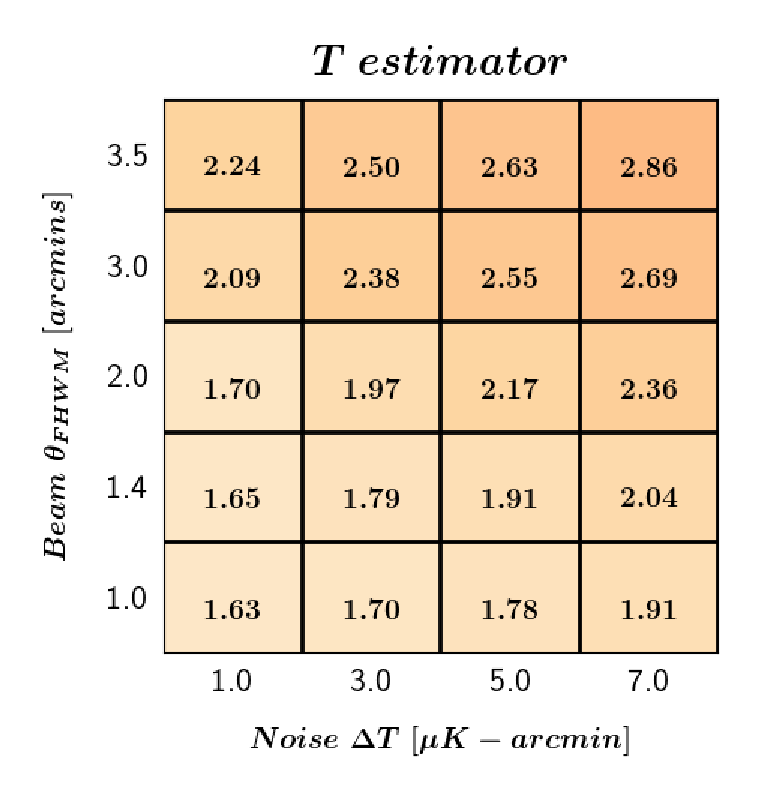
\includegraphics[width=0.46\textwidth, height=0.5\textwidth,clip=]{figs/fig4.eps}
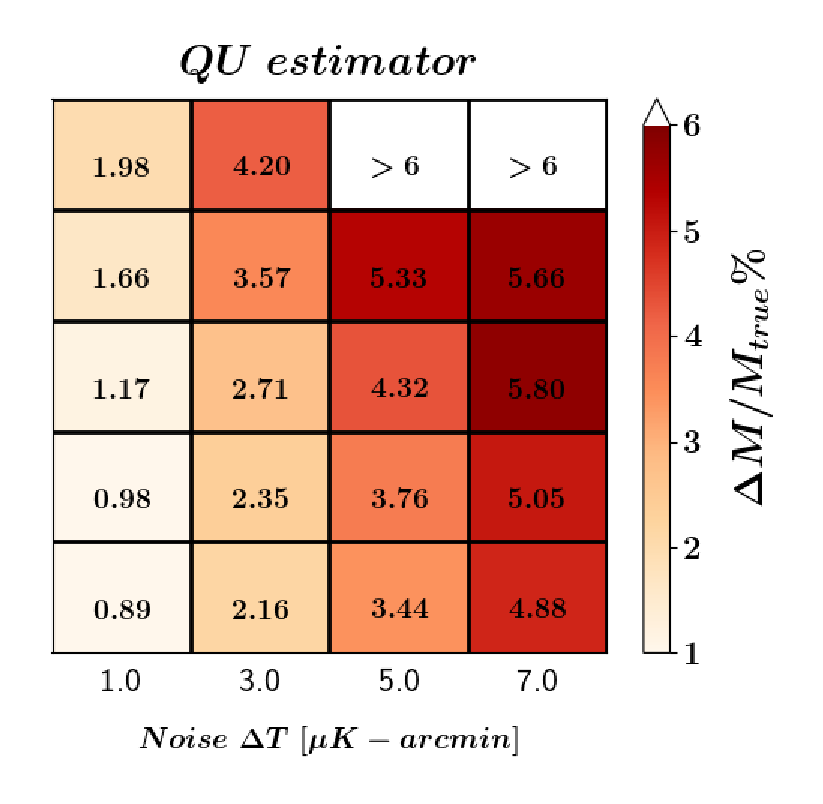
\includegraphics[width=0.5\textwidth, height=0.5\textwidth,clip=]{figs/fig5.eps}
\caption{The performance of the polarization MLE is very sensitive both to the angular resolution and map noise level of an experiment; the gains for the temperature MLE are much smaller. The numbers correspond\
 to the CMB-cluster lensing mass uncertainty (in percent) of the cluster sample containing 100,000 clusters after the addition of foregrounds (dotted lines in right panel of Fig. \ref{fig_delM_M_1000_clusters_T_QU_EB_ideal_FG}).
Improving the beam from $3.'5$ to $1'$ enhances the SNR by a factor of two for the CMB-S4 noise levels.
The saturation of $T_{\rm ML}$ is due to the larger impact of foregrounds on the temperature maps. }
\label{fig_beam_dependency_T_QU}
\end{figure*}

To provide realistic estimates of the mass uncertainties, we perform a constrained internal linear combination (ILC) of data from 90, 150, and 220 GHz channels based on the \texttt{SMICA} (Spectral Matching Ind\
ependent Component Analysis) algorithm \citep{smicacardoso, PLANCKCOMPSEP2014} to eliminate the tSZ signal from the temperature data and minimize the residual power in other extragalactic foregrounds and instru\
mental noise in both temperature and polarization.
The resulting power spectra of the instrumental noise and residual foregrounds for different CMB experiments are shown in Fig.~\ref{fig_ILC_res}.
At $\ell \le 2000$, the temperature curves are dominated by residual foreground power as three frequency bands are insufficient to completely eliminate the foreground power in the assumed model (see Appendix).
As a result, the temperature noise curves  converge at $\ell \le 2000$ despite the very different noise levels of the  experiments.
During this process, we convolve the 90 and 220 GHz spectra by the ratio of 150 GHz beam and their native beams, so that the final effective beam size matches 150 GHz.

The expected performance of each  experiment is given in Table \ref{tab_forecast_future_CMBexp}.
One significant uncertainty is the number of clusters to assume for each experiment.
As accurately modeling the survey selections functions for SZ, optical, and X-ray surveys is beyond the scope of this work, we make the simplifying assumption that all Stage III experiments will have 10,000 clu\
sters and the CMB-S4 experiment will have 100,000 clusters.
%This is of order the number expected to be discovered through the tSZ effect by the SPT-3G (8000 clusters; \citet{benson2015_3g}) or AdvACT (10,000 clusters; \citet{advact_2016}), but likely an over-estimate f\
or the Simons Array due to its larger 3.5$^\prime$ beam size.                                                                                                                                                      
This is of order the number expected to be discovered through the tSZ effect by the SPT-3G or AdvACT (see above), but likely an over-estimate for the Simons Array due to its larger 3.5$^\prime$ beam size.
On the other hand, the experimental beam size is irrelevant when predicting the size of cluster samples from optical or X-ray surveys that overlap with the CMB surveys.
The DES or LSST surveys should provide samples with more than 50,000 clusters for all of the Stage III CMB experiments \citep{rykoff2016, lsst_science_book}.
Given a specific sample size, the mass uncertainty can be obtained by rescaling the numbers provided in Table \ref{tab_forecast_future_CMBexp} by $\sqrt{\frac{N_{sample}}{N_{clus}}}$.

Even considering concerns about potential biases from astrophysical signals, the temperature channel will be extremely important for the cluster mass estimates from the Stage III CMB experiments.% (AdvACT, Simo\
ns Array, SPT-3G).
 The mass uncertainty on the fiducial 10,000 cluster sample  is similar in temperature from all three experiments, with a range from 3.3\% (SPT-3G) to 5.9\% (the Simons Array wide survey). These uncertainties ar\
e as large as the likely systematic uncertainties, and the statistical uncertainties on polarization are higher by a factor of two or more. As an example of scaling the results with sample size, we replace the \
fiducial sample size by the expected number counts for SZ-discovered clusters with SPT-3G (8000) and optically detected clusters from the DES (50,000). SPT-3G would achieve a 3.6\% mass uncertainty with a sampl\
e of 8000 SZ-selected clusters and a 1.5\% uncertainty on a sample of 50,000 optically-selected clusters. The shallow portions of the Simons Array or AdvACT surveys cannot contribute much for the polarization e\
stimator; lower noise levels are essential. The polarization estimator can be within a factor of two for the deep surveys of the Simons Array or SPT-3G. For instance, the polarization estimator for SPT-3G on 80\
00 clusters yields a 6.8\% mass calibration, to be compared to the 3.6\% mass calibration from temperature (ignoring systematic uncertainties).


The lower level of systematic uncertainty for polarization comes into play for the CMB-S4 experiment. First, for the extremely low noise levels of CMB-S4, the performance of the temperature and polarization cha\
nnels is nearly identical (0.95\% vs.~0.98\%) for an instrument with $2'$ beam resolution. Second, the magnitude of the temperature-only systematic errors (primarily from the SZ effect) is now several times lar\
ger than the raw statistical uncertainties, and would dominate the temperature error budget. We can expect cluster mass calibrations from CMB-S4's polarization data at the 1\% level.

The mass calibration forecasts in  Table \ref{tab_forecast_future_CMBexp} are highly complementary  to and competitive with the masses obtained by stacking optical weak lensing measurements. For example, LSST h\
opes to achieve a mass uncertainty of 1\% by stacking few thousands of clusters at redshifts $z < 0.5$ \citep{lsst_science_book}. At high redshifts, since the number density of background galaxies decrease rapi\
dly, the constraints from optical lensing measurements tend to weaken. Calibrating the high redshift end of the mass function is the true power of CMB-cluster lensing which will allow us to place important cons\
traints on the redshift evolution of mass-observable scaling relations out to high redshifts $z \ge 1.5$.